\documentclass{article}

\usepackage{graphicx}
\usepackage{tikz}
\usepackage{tikzsymbols}
\usetikzlibrary{calc,patterns,shapes.geometric}
\pagestyle{empty}
\usepackage[margin=0pt]{geometry}
\geometry{papersize={14in,12in}}

\def\centerarc[#1](#2)(#3:#4:#5){\draw[#1] ($(#2)+({#5*cos(#3)},{#5*sin(#3)})$) arc (#3:#4:#5);}

\begin{document}
	\begin{figure}
		\centering
		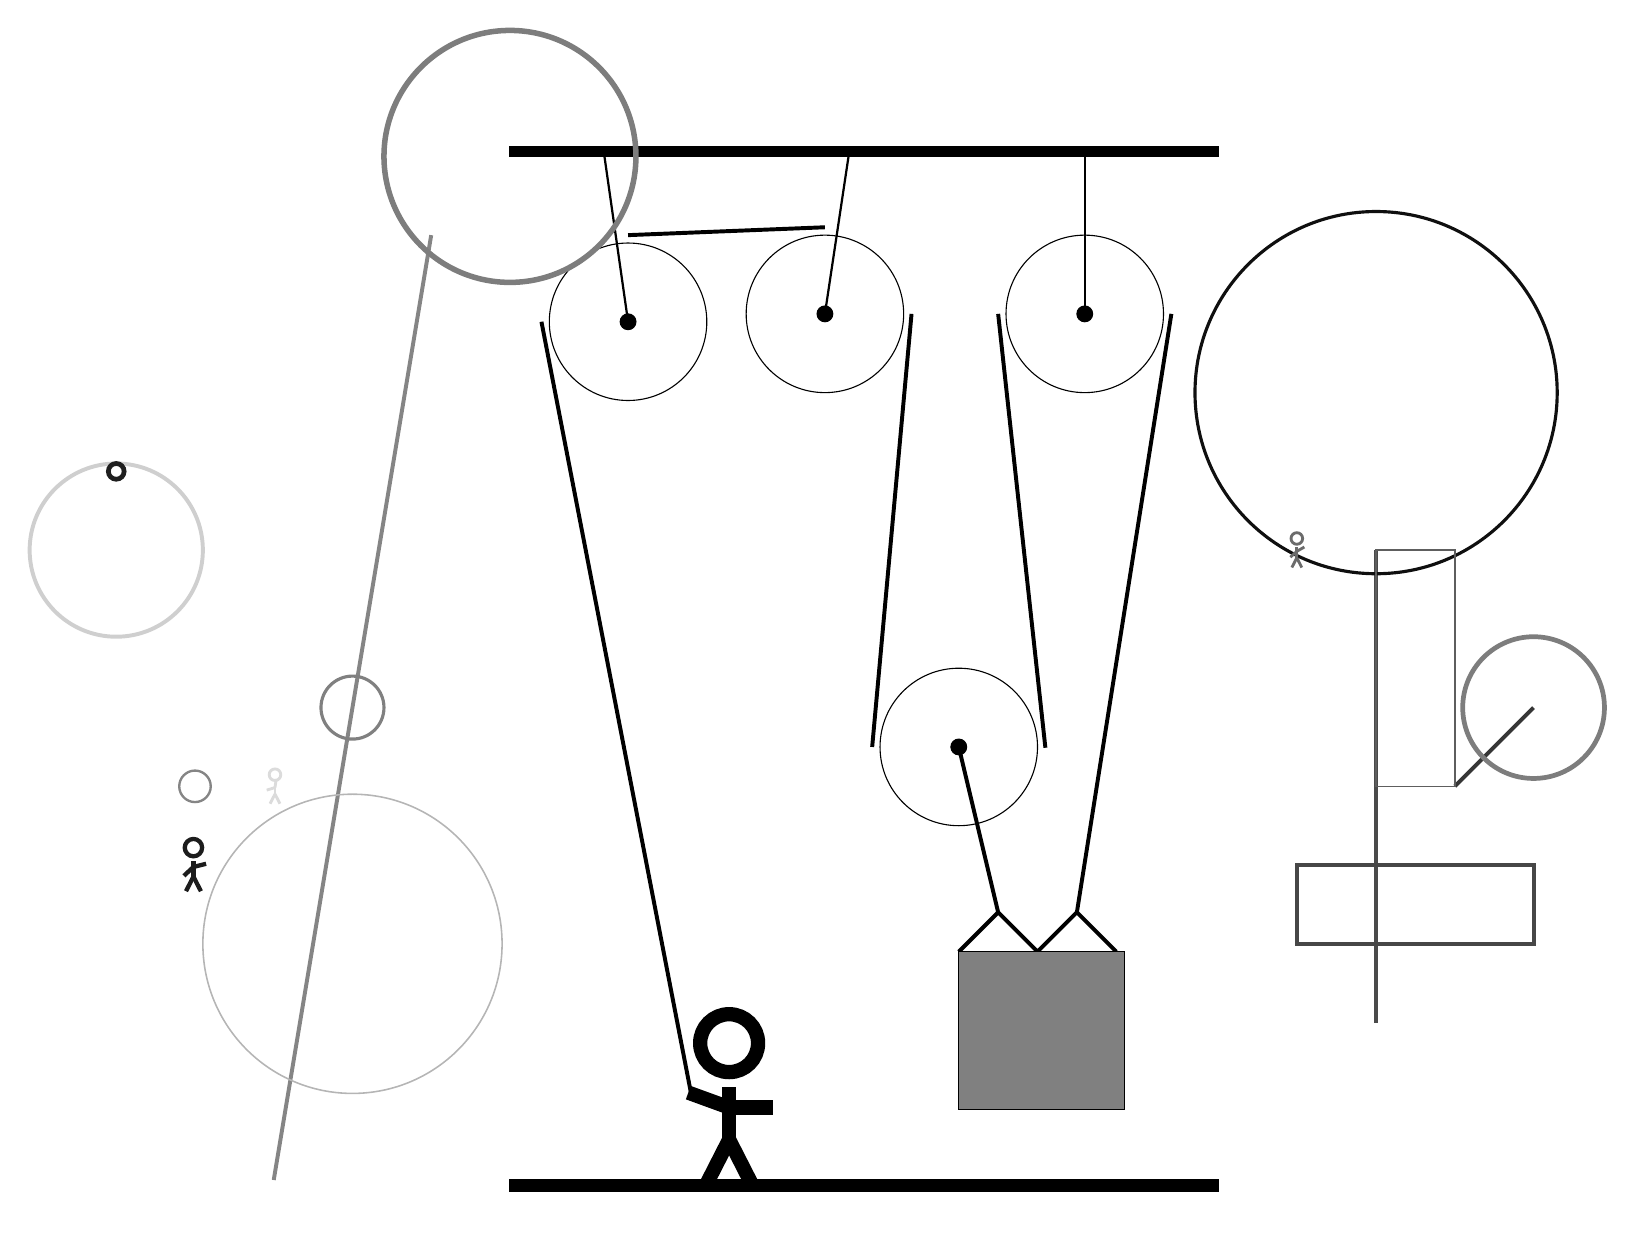
\begin{tikzpicture}
			%%%%% START %%%%%
			
			\draw[fill=black] (-3, 10) rectangle (6, 10.125);
			
			\draw (1, 8.0) circle (1);
			\draw[fill=black] (1, 8.0) circle (0.1);
			\draw[thick] (1, 8.0) -- (1.3, 10);
			
			\draw (4.3, 8.0) circle (1);
			\draw[fill=black] (4.3, 8.0) circle (0.1);
			\draw[thick] (4.3, 8.0) -- (4.3, 10);
			
			\draw (2.7, 2.5) circle (1);
			\draw[fill=black] (2.7, 2.5) circle (0.1);
			
			\draw[line width=0.5mm]  (2.7, -0.1) -- (3.2, 0.4) -- (3.7, -0.1) -- (4.2, 0.4) -- (4.7, -0.1);
			\draw[fill=black!50] (2.7, -0.1) rectangle (4.8, -2.1);
			
			\draw (-1.5, 7.9) circle (1);
			\draw[fill=black] (-1.5, 7.9) circle (0.1);
			\draw[thick] (-1.5, 7.9) -- (-1.8, 10);
			
			\draw[line width=0.5mm](-0.7, -1.9) --  (-2.6, 7.9);
			\centerarc[line width=0.5mm](-1.5, 7.9)(90:180:1.1);
			\draw[line width=0.5mm](-1.5, 9.0) -- (1, 9.1);
			\centerarc[line width=0.5mm](1, 8.0)(0:90:1.1);
			\draw[line width=0.5mm](2.1, 8.0) -- (1.6, 2.5);
			\centerarc[line width=0.5mm](2.7, 2.5)(180:370:1.1);
			\draw[line width=0.5mm] (3.8, 2.49) -- (3.2, 8.0);
			\centerarc[line width=0.5mm](4.3, 8.0)(0:180:1.1);
			\draw[line width=0.5mm](4.2, 0.4) -- (5.4, 8.0);
			\draw[line width=0.5mm] (3.2, 0.4) -- (2.7, 2.5);
			
			\draw[line width=0.5mm, color=black!48](-4, 9) -- (-6, -3);
			
			\draw[line width=0.5mm, color=black!71](8, -1) -- (8, 5);
			\draw [line width=0.5mm, color=black!19](-8, 5) circle (1.1);
			\draw [line width=0.4mm, color=black!50](-5, 3) circle (0.4);
			\draw [line width=0.4mm, color=black!94](8, 7) circle (2.3);
			
			\node[line width=0.5mm, color=black!89] at (-7, 1) {\Strichmaxerl[3][43][14]};
			
			\draw [line width=0.2mm, color=black!29](-5, 0) circle (1.9);
			\draw[line width=0.5mm, color=black!79](9, 2) -- (10, 3);
			\draw [line width=0.7mm, color=black!51](-3, 10) circle (1.6);
			\draw [line width=0.3mm, color=black!48](-7, 2) circle (0.2);
			\draw[line width=0.2mm, color=black!63] (8, 5) rectangle (9, 2);
			\draw [line width=0.6mm, color=black!88](-8, 6) circle (0.1);
			\node[line width=0.6mm, color=black!58] at (7, 5) {\Strichmaxerl[2][42][30]};
			\draw [line width=0.6mm, color=black!51](10, 3) circle (0.9);
			\draw[line width=0.5mm, color=black!72] (7, 1) rectangle (10, 0);
			\node[line width=0.7mm, color=black!14] at (-6, 2) {\Strichmaxerl[2][17][82]};
			
			
			\node at (-0.2, -2) {\Strichmaxerl[10][-20][0]};
			
			\draw[fill=black] (-3, -3) rectangle (6, -3.15);
			
			%%%%% END %%%%%
		\end{tikzpicture}
	\end{figure}	
\end{document}